\documentclass[12pt,a4paper]{article}
\usepackage[utf8]{inputenc}
\usepackage[french]{babel}
\usepackage[T1]{fontenc}
\usepackage{amsmath}
\usepackage{amsfonts}
\usepackage{amssymb}
\usepackage{graphicx}
\usepackage{url}
\usepackage[usenames,dvipsnames]{xcolor}
\usepackage[colorlinks=false,urlbordercolor=white,linkbordercolor=white]{hyperref}
\usepackage[left=2cm,right=2cm,top=2cm,bottom=3cm]{geometry}
\usepackage{fancyhdr}
\usepackage{lmodern}
\usepackage{listings}
\pagestyle{fancy}
\usepackage{titlesec}
\usepackage[abs]{overpic}
\usepackage{tabularx}
\usepackage{times}
\usepackage{graphicx}

% gestion de la police sans-serif (helvetica, équivalent arial) :
% décommenter les deux lignes suivantes
%\usepackage{helvet}
%\renewcommand{\familydefault}{\sfdefault}

% Definition de l'affichage du code
\lstset{breaklines=true,basicstyle=\footnotesize\ttfamily,frame=single, numbers=left
%,backgroundcolor=\color{lightgray}
}

% Definition des couleurs
\definecolor{titreColor}{RGB}{0,58,128}  % Marine
\definecolor{stitreColor}{RGB}{0,158,224}  % Ocean
\definecolor{auteurColor}{RGB}{0,58,128}     % Marine
\definecolor{texteColor}{RGB}{164,196,0}     % Prairie

% Definition du sommaire
\usepackage[tight]{shorttoc}
\newcommand{\sommaire}{\shorttoc{Sommaire}{2}}

% Definition des chapitres
\titleformat{\section}
{\color{titreColor}\normalfont\Large\bfseries\sffamily}
{\color{titreColor}\thesection}{1em}{}

\titleformat{\subsection}
{\color{stitreColor}\bfseries\sffamily}
{\color{stitreColor}\thesubsection}{1em}{}

%Données de titre et d'auteur pour la page de garde
\newcommand{\titre}{Projet USACT}
\newcommand{\sousTitre}{Diagramme des cas d'utilisation}
\newcommand{\auteur}{Jérémy DAMEY}
\newcommand{\dateModif}{\today}


\begin{document}
%Supprime les veuves et orphelines
\widowpenalty=10000
\clubpenalty=10000
\raggedbottom 

%entete
\fancyhead{}
\renewcommand{\headrulewidth}{0pt}
%pied de page
\fancyfoot{}
\fancyfoot[C]{\sffamily\thepage}
\fancyfoot[L]{\textcolor{titreColor}{\sffamily\textbf{IRSTEA} - Centre de Bordeaux\\}
\fancyfoot[R]{\textcolor{auteurColor}{\sffamily\auteur{}}\\{\sffamily\dateModif{}}}
\textcolor{stitreColor}{\sffamily 50, avenue de Verdun, Gazinet\\
33612 CESTAS Cedex }}
\fancyfoot[R]{\sffamily\author{}}

% Insertion du logo, du titre et du sous-titre
\begin{minipage}{0.2\linewidth}

\includegraphics[width=3.06cm,height=9.57cm,keepaspectratio]{Image/logo_irstea}%
\end{minipage}
\hspace{0.1cm}
\begin{minipage}{0.8\linewidth}
\LARGE\flushleft \color{titreColor}{\bfseries\sffamily\titre{}}\\
\large\flushleft \color{stitreColor}{\bfseries\sffamily\sousTitre{}}
\end{minipage}

\vspace{1cm}
\section{Présentation}

Cette application a été, initialement, conçu pour gérer les conflits d'usage au sein du bassin d'Arcachon. L’étude des conflits s’appuie sur une méthodologie développée par Torre et al. (2010), \emph{comment évaluer et mesurer la conflictualité liée aux usages de l'espace ? Eléments de méthode et de repérage.} \newline \newline
L'étude des conflits est basée sur l’utilisation de trois sources de données complémentaires :
\begin{description}
\item[–	La Presse Quotidienne Régionale  (PQR) ,] pour accéder à une information locale détaillée;
\item[–	Les entretiens auprès d’experts ,] pour recueillir des informations auprès d’experts locaux, impliqués ou non dans les conflits; 
\item[–	Les relevés de contentieux ,] permettant de recenser les conflits qui font l’objet d’un  traitement juridique. \newline
\end{description}


Initialement créée sous ACCESS, la base de données a été migrée vers un serveur de base de données en PostGreSQL. L’interface de saisie est alors devenue inadaptée. Le but est de faciliter l’accès aux données pour les chercheurs impliqués dans un projet. L'objectif est qu'il est l'accès aux données en lecture et en écriture. \newline \newline

Les chercheurs ont la possibilité de pouvoir travailler sur trois domaines différents, à savoir Arcachon, Marseille et l'Île de la Réunion.\newline
\underline{Domaine :} C'est une zone géographique d'étude pour les chercheurs.

Les données sont organisées en domaine d'études, c'est-à-dire en zone géographique restreinte et homogène pour étudier les conflits d'usage. L'application devra permettre aux chercheurs de travailler dans trois domaines : Arcachon, Marseille et l'Île de la Réunion.

\clearpage
\begin{figure}
\section{Diagramme des cas d'utilisation}
\vspace{0.5cm}
\centering
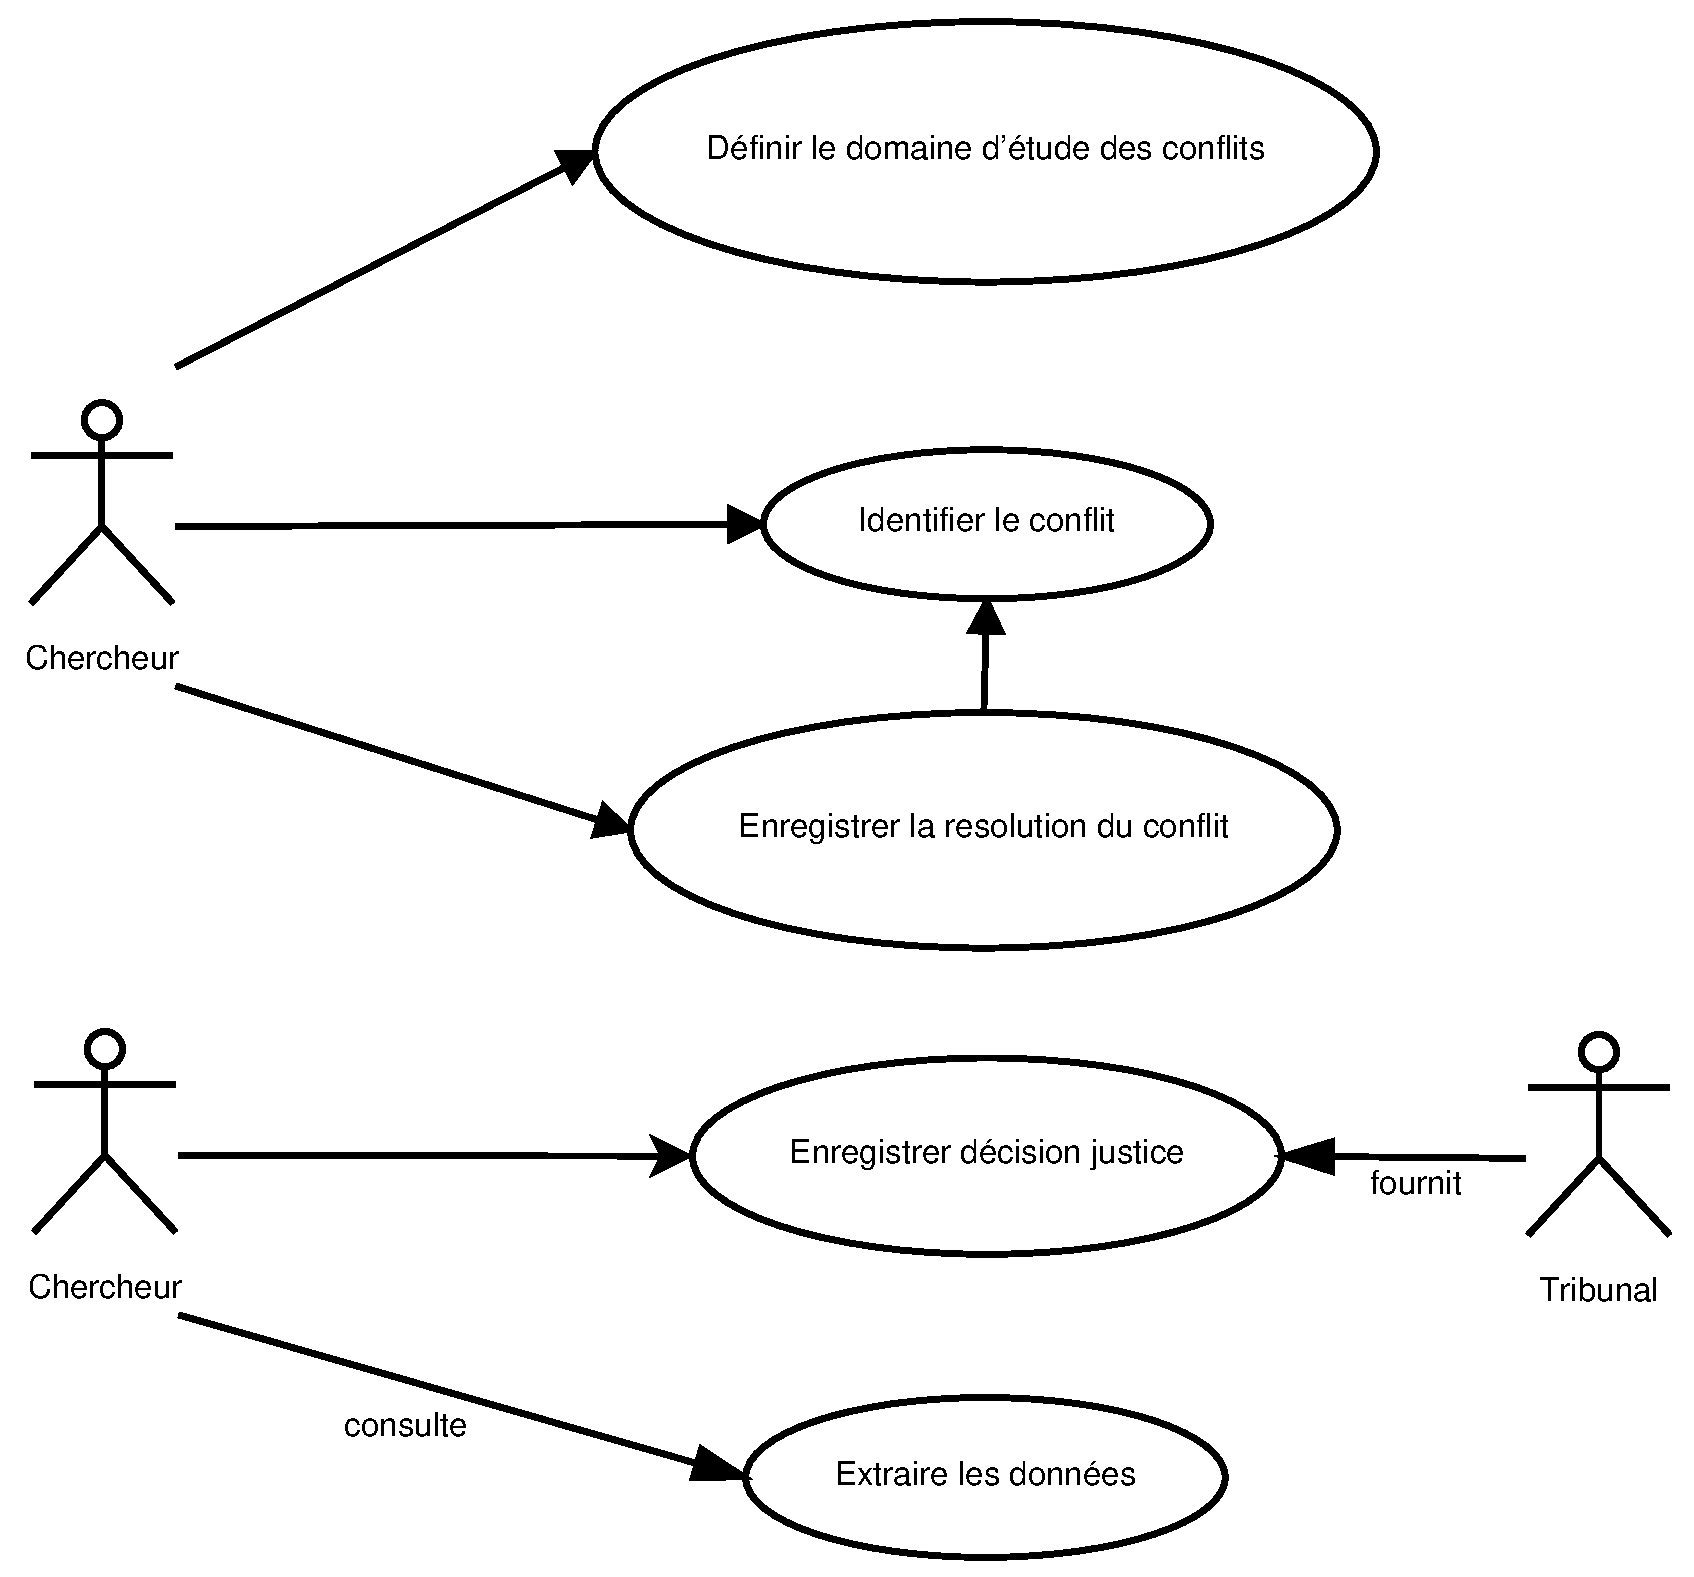
\includegraphics[width=\textwidth]{Image/CU.eps}
\caption{Diagramme des cas d'utilisation}
\end{figure}

\vspace{1cm}
\subsection{Les acteurs}
\begin{description}
\item[Le chercheur :]C'est l'utilisateur de l'application. Chaque chercheur a le même rôle au sein de l'application. 
\item[Le tribunal :] Son rôle est de prendre les décisions concernant les conflits, c'est-à-dire donner son avis concernant la résolution de celui-ci. \newline
Le tribunal peut représenter plusieurs parties, à savoir le Conseil d'État, la Cour administrative d'appel, la Cour de cassation et la Cour d'appel.
\end{description}


\subsection{Définir le domaine d'étude des conflits}
Trois domaines d'étude à l'IRSTEA : Arcachon, Marseille et l'Île de la Réunion. 
Les chercheurs sont habilités à travailler sur un ou plusieurs domaines.

\subsection{Identifier le conflit}
Un conflit à l'expression d'un problème entre 2 ou plusieurs acteurs dans une zone géographique bien délimitée dans un domaine d'étude précisé. \newline 
Un conflit est identifié par :
\begin{description}
\item[Les sources de données :] informations sur la source de données
\item[Les matérialités du conflit :] informations sur le bien support, l’objet du conflit
\item[Le genèses et déroulement du conflit :] période, localisation, résolution 
\item[Les acteurs du conflit :] informations sur les personnes (physiques et/ou morales) qui participent au conflit
\item[Les interventions des acteurs dans le conflit :] rôle de l’acteur, lien avec la matérialité du conflit, motifs de revendication et types d’arguments invoqués, mode d’action, solution proposée \newline \newline
\end{description}

\begin{figure}[!ht]
\centering
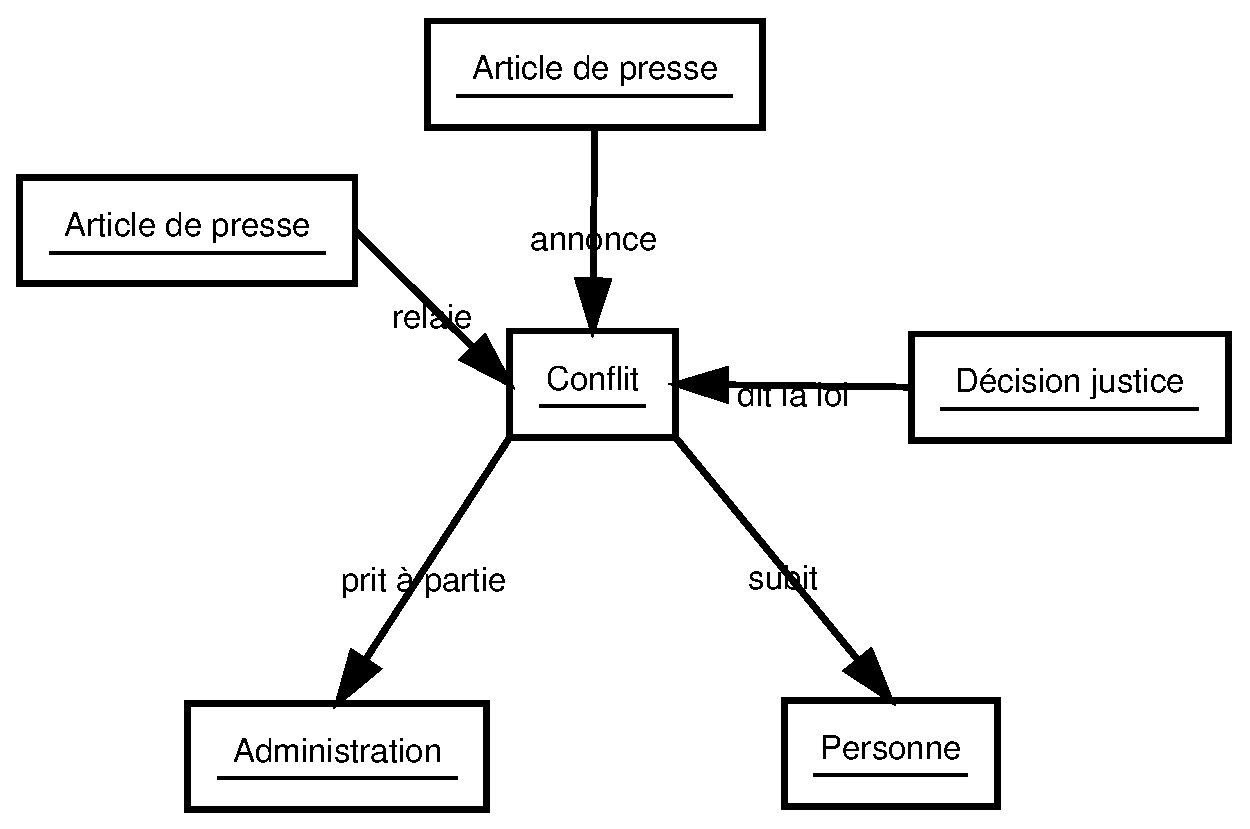
\includegraphics[width=\textwidth]{Image/ExplicationConflit.eps}
\caption{Diagramme de la description d'un conflit}
\end{figure}

Avant que l'on parle de la déclaration d'un conflit, il faut avoir au moins une source relatant l'information. Sur ce schéma explicatif, nous avons 2 sources de données, à savoir 2 articles de presse. L'un annonce ou parle du conflit et l'autre relaie l'information à ce sujet. Une fois la ou les sources déclarées, nous avons la création de notre conflit. Nous avons la justice qui travaille sur ce conflit pour annoncer le verdict. Enfin, quand il y a un conflit, il y a une ou plusieurs personnes qui subissent les faits et il peut également y avoir une partie administrative qui est prise à partie. \newline

% Insertion d'une tabulation
\begin{description}
\item[Identifier les acteurs :] Les acteurs sont des personnes contestataires, c'est-à-dire des personnes qui sont en désaccord avec une décision qui a été prise. 
\item[Identifier les sources :] Trois sources d'informations sont disponibles. Nous avons \textit{la presse} qui donne des informations à travers les journaux, \textit{les entretiens avec les experts}, cela permet d'avoir un apport d'informations supplémentaires par rapport à ce qui a été dit dans la presse, \textit{le contentieux}, c'est-à-dire la décision qui a été prise au tribunal suite à la contestation d'un ou des acteurs. \newline
\end{description}

\clearpage
\begin{figure}[!h]
\centering
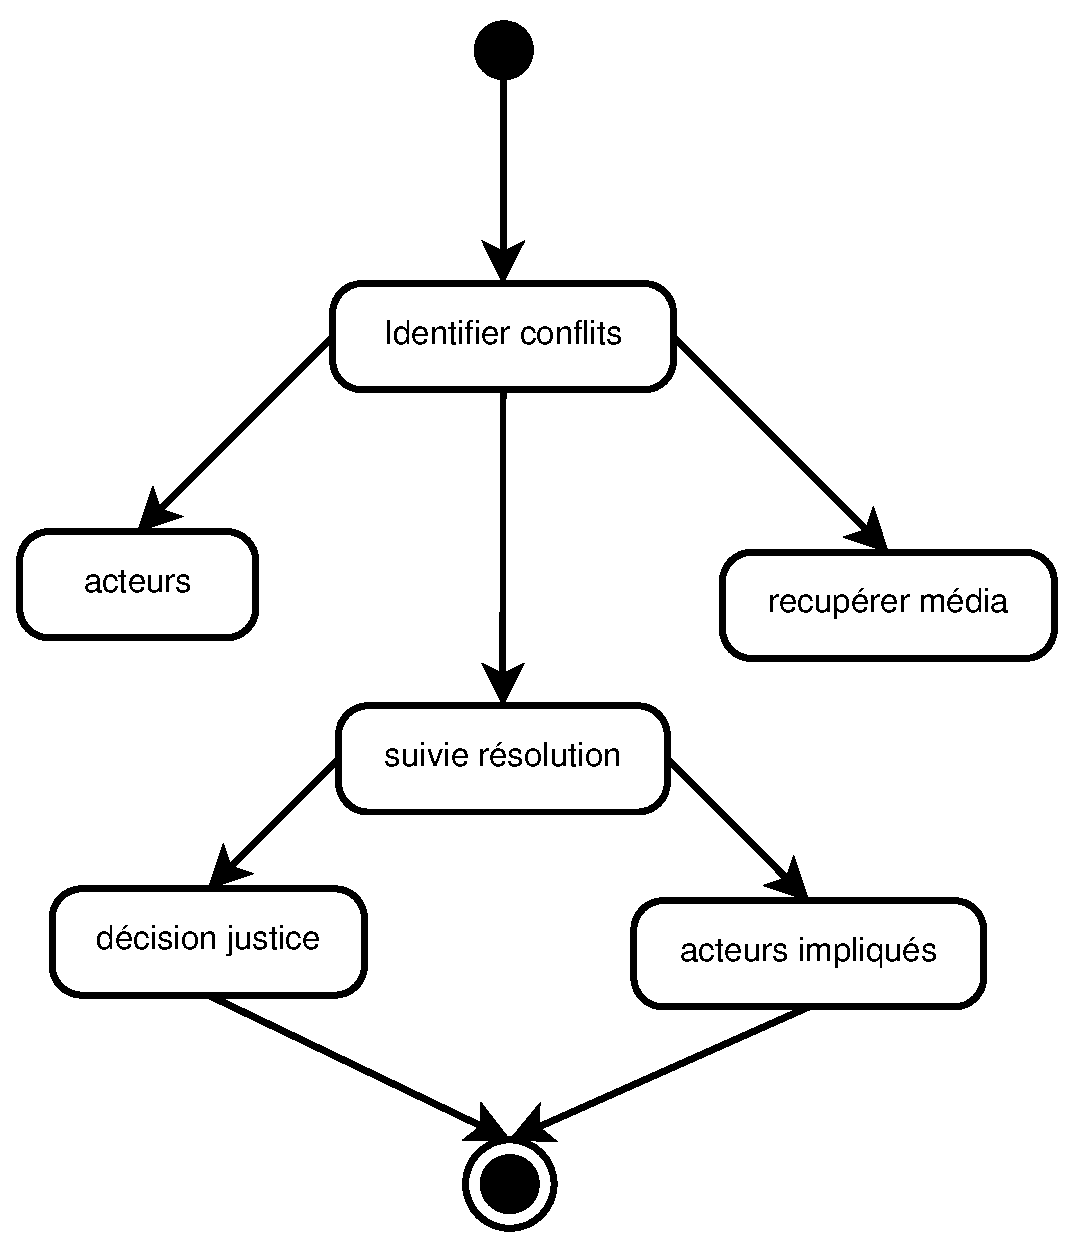
\includegraphics[width=\textwidth]{Image/diagrammeConflit.eps}
\caption{Diagramme de suivi du déroulement d'un conflit}
\end{figure}

Sur ce schéma, nous avons tout d'abord l'identification du conflit. Une fois le conflit identifié, nous déterminons les acteurs qui sont à l'origine du conflit mais également les médias, c'est-à-dire la presse, les entretiens et le contentieux. Il faut également suivre la résolution de celui-ci, c'est-à-dire l'état d'avancement, les idées proposées pour trouver un arrangement entre les parties qui sont en désaccord. Enfin, il peut y avoir une décision de la justice qui va indiquer quels sont les acteurs gagnants. 

\subsection{Enregistrer la résolution du conflit}
La résolution d'un conflit correspond à l'état d'avancement, c'est-à-dire à l'élaboration d'idées pour trouver une entente entre les acteurs qui sont en désaccord. C'est la partie où le chercheur va enregistrer les résultats élaborés par les différents acteurs.

\subsection{Extraire les données}
L'extraction des données, à l'heure actuelle, n'est pas tout à fait définie. 
Les chercheurs ont besoin d'accéder aux informations pour les traités, 
Ce sont donc des suppositions intéressantes pour le chercheur que nous allons établir. Cela pourrait donc servir à consulter les données stocker dans la base en l'interrogeant, consulter les statistiques à travers des graphiques générer automatiquement... Plusieurs possibilités pourraient également être proposées.

\subsection{Enregistrer les décisions de justice}
C'est la partie clé du conflit, c'est ici que nous tenons compte de la décision prise par la justice pour rétablir l'ordre au sein de ce conflit. C'est la justice qui dicte la loi, par conséquent, c'est elle qui a le dernier mot.


% Insertion du sommaire
% \sommaire
%\tableofcontents

% Debut effectif du texte

\end{document}